\chapter{Développement}
\label{chapter:dev}

\label{chapitre4}
		
		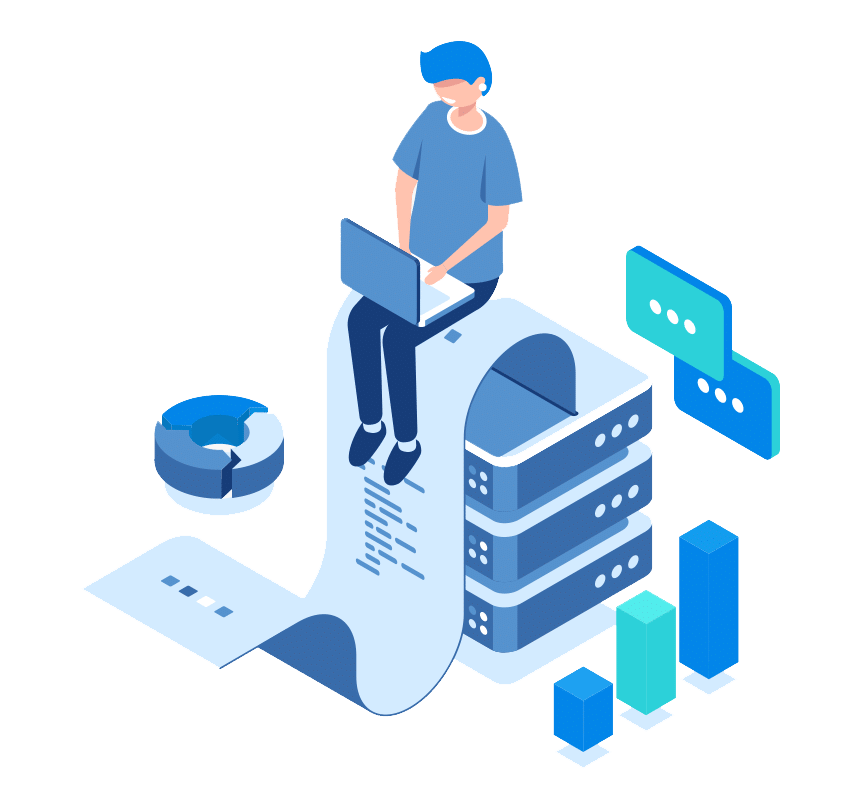
\includegraphics [width=1 \linewidth, height=0.8\textheight, keepaspectratio] {Images/chapterFigures/chFour.png}
		
	
		
		\newpage

Après avoir expliqué notre approche dans le chapitre précédent, dans ce chapitre nous expliquerons en détail comment le système proposé met en œuvre l'approche et comment elle fonctionne.

\section{Architecture du système}

Notre système se compose de plusieurs parties; une application mobile qui recueille des données, un serveur où les données en cours de traitement et stocke le résultat du traitement dans une base de données, une copie des données vers le DTP et enfin une carte interactive avec l'état de la route en temps réel pour les conducteurs.

\subsection{Aperçu de système}
\begin{figure}[h!]
    \center
    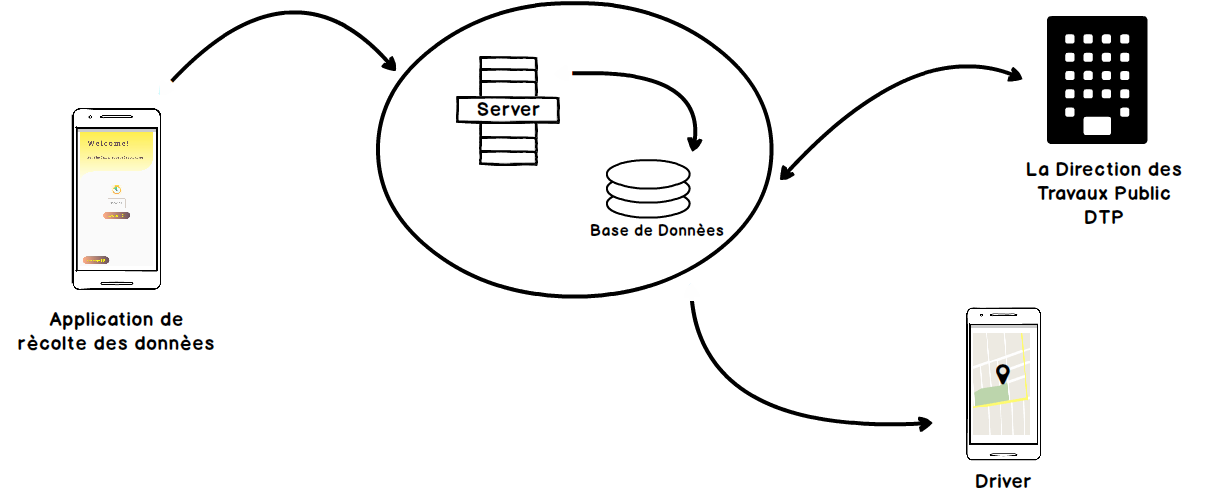
\includegraphics[width=0.75\textwidth]{Images/chapter3/systemOverview.png}
    \caption{Un aperçu du système proposé.}
    \label{fig:System}
\end{figure}

\begin{itemize}
    \item \textbf{Application de rècolte des donnèes:} Une application mobile où les capteurs du smartphone sont utilisés pour collecter les données du journal de conduite et envoyer les données au serveur.
    \item  \textbf{Server:} Après avoir reçu les données, le serveur estime l'état de la route et enregistre les résultats dans une base de données.
    \item \textbf{Base de donnèes:} Il contient les résultats estimés de l'état de la route et l'enregistre pour être desservi par d'autres parties.
    \item  \textbf{DTP:} La Direction des Travaux Publics; la partie principale qui utilise les résultats de la base de données. Nous pouvons étendre ce système avec une application de tableau de bord pour eux, qui: \begin{itemize}
              \item Leur permettre de surveiller régulièrement l'état de la route pour prendre plus rapidement des décisions d'entretien et de réparation.
              \item Envoyez les données fixes sur l'état de la route à la base de données après la réparation.
          \end{itemize}
    \item \textbf{Driver:} Nous pouvons également étendre ce système avec une application mobile, qui fournit au conducteur moyen une carte interactive montrant les conditions routières actuelles pour une meilleure expérience de conduite.
\end{itemize}

\subsection{Fonctionnement de système}
\begin{figure}[ht]
    \center
    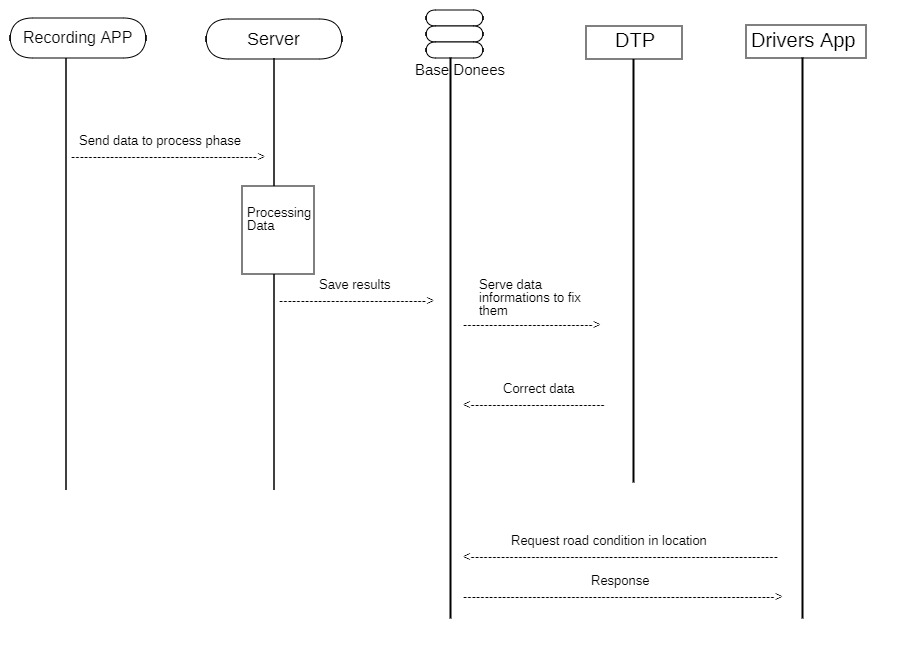
\includegraphics[width=1.2\textwidth]{Images/chapter3/diagrameSequence.jpg}
    \caption{Diagramme de séquence}
    \label{fig:System}
\end{figure}

Notre système sous forme de diagramme montre l'envoi des données du journal de collecte de l'application d'enregistrement au serveur sous forme de fichier CSV, dès qu'il existe; Le serveur facture l'étape du processus d'enregistrement des résultats dans la base de données.

L'application de tableau de bord DTP utilise la base de données pour corriger les défauts, tandis que l'application Driver l'utilise pour une meilleure expérience du conducteur.



\section{Technologies utilisées}
\subsection{Python}
Python \cite{WelcomePythonOrg} est un langage de programmation qui peut s'utiliser dans de nombreux contextes et s'adapter à tout type d'utilisation grâce à des bibliothèques spécialisées. Il est cependant particulièrement utilisé comme langage de script pour automatiser des tâches simples mais fastidieuses. On l'utilise également comme langage de développement de prototype lorsqu'on a besoin d'une application fonctionnelle avant de l'optimiser avec un langage de plus bas niveau. Il est particulièrement répandu dans le monde scientifique, et possède de nombreuses bibliothèques optimisées destinées au calcul numérique \cite{PythonLangageWikipedia}.
\renewcommand{\labelitemi}{$\bullet$}

\paragraph{Pandas:}
Pandas \cite{PandasPythonData} est une bibliothèque écrite pour le langage de programmation Python permettant la manipulation et l'analyse des données. Elle propose en particulier des structures de données et des opérations de manipulation de tableaux numériques et de séries temporelles. Pandas est un logiciel libre sous licence BSD.

Les principales structures de données sont les séries (pour stocker des données selon une dimension - grandeur en fonction d'un index), les DataFrames (pour stocker des données selon 2 dimensions - lignes et colonnes), les Panels (pour représenter des données selon 3 dimensions, les Panels 4D ou les Data Frames avec des index hiérarchiques aussi nommés Multi Index (pour représenter des données selon plus de 3 dimensions - hypercube) \cite{Pandas2020}.


\begin{figure}[h!]
    \center
    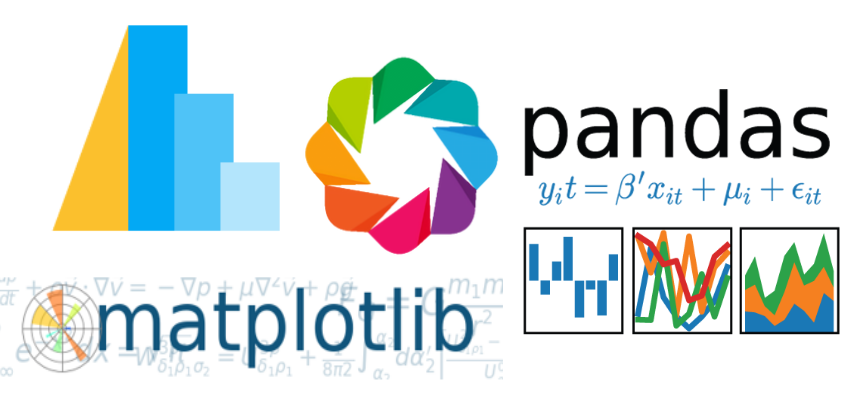
\includegraphics[width=0.50\textwidth]{Images/chapter3/python_pandas.png}
    \caption{Python and Pandas Logos}
    \label{fig:Technologies}
\end{figure}

\subsection{REST API}
API est une abréviation de:  Application Programming Interface (ou interface de programmation d’application, en français). Pour faire simple : c’est un moyen de communication entre deux logiciels, que ce soit entre différents composants d’une application ou entre deux applications différentes.

REST signifie Representational State Transfer (ou transfert d’état de représentation, en français), et constitue un ensemble de normes, ou de lignes directrices architecturales qui structurent la façon de communiquer les données entre votre application et le reste du monde, ou entre différents composants de votre application.

Nous utilisons l’adjectif RESTful pour décrire les API REST. Toutes les API REST sont un type d’API – mais toutes les API ne sont pas RESTful.Les API RESTful se basent sur le protocole HTTP pour transférer les informations – le même protocole sur lequel la communication web est fondée \cite{IdentifiezAvantagesAPI}.


\subsection{Flask}
Flask \cite{WelcomeFlaskFlask} est un framework open-source de développement web en Python. Son but principal est d'être léger, afin de garder la souplesse de la programmation Python, associé à un système de templates.
Flask a été créé initialement par Armin Ronacher comme étant un poisson d’Avril. Le souhait de Ronacher était de réaliser un framework web contenu dans un seul fichier Python mais pouvant maintenir des applications très demandées.
En 2018, Flask était élu "Framework web le plus populaire" par le Python Developers Survey. En janvier 2020, il cumulait plus de 49000 étoiles sur Github, plus que n'importe quel autre framework de développement web Python\cite{FlaskFramework2020}.
\begin{figure}[h!]
    \center
    
\includegraphics[width=0.50\textwidth]{Images/chapter3/flask.png}
    \caption{Logo Flask}
    \label{fig:Technologies}
\end{figure}

\subsection{Flutter}
Flutter \cite{FlutterBeautifulNative} est un SDK pour applications mobiles permettant de créer des applications hautes performances et haute fidélité pour iOS et Android à partir d’une seule base de code.
L’objectif est de permettre aux développeurs de proposer des applications hautes performances qui se sentent naturelles sur différentes plates-formes.

Comme React Native, Flutter fournit également des vues de style réactif. Flutter adopte une approche différente pour éviter les problèmes de performances causés par la nécessité d’un pont JavaScript en utilisant un langage de programmation compilé, à savoir Dart \cite{rahmouniBindex}.
\renewcommand{\labelitemi}{$\bullet$}
\begin{itemize}
    \item \textbf{\textit{Dart:}}

          Dart est un langage de programmation polyvalent développé à l’origine par Google et ensuite approuvé en tant que norme par Ecma (ECMA-408). Il est utilisé pour créer des applications Web, serveur, bureau et mobiles.
          Dart est un langage basé sur les objets, orienté objet, défini par la classe et utilisant une syntaxe de style C qui transcompile éventuellement en JavaScript. Il prend en charge les interfaces, mixins, classes abstraites, génériques réifiés, typage statique et un système de type sonore \cite{WhatRevolutionaryFlutter}.
\end{itemize}
\begin{figure}[h!]
    \center
    
\includegraphics[width=0.50\textwidth]{Images/chapter3/flutter.png}
    \caption{Flutter Logo}
    \label{fig:Technologies}
\end{figure}





\section{Application de collecte}
\label{sec:app_record}
Nous avons développé une application mobile utilisant Flutter pour la collecte de données à l'aide des capteurs de téléphone.
\begin{itemize}
    \item D'abord, l'application demande à l'utilisateur d'entrer la durée d'enregistrement en minutes - Montre en capture d'écran «par seconde» à des objectifs du test - (Figure \ref{fig:Welcome Screen}).
          
    \item Deuxièmement, il lui demande d'activer le GPS (Figure \ref{fig:GpsAcivate}). Sinon, il ne démarrera pas l'enregistrement (Figure \ref{fig:gpsNotif}).



    \item Une fois le GPS activé et l'heure d'enregistrement entrée, l'application amène l'utilisateur à l'écran d'enregistrement, lui montrant une carte en temps réel et un graphique accéléromètre / gyroscope. Il peut annuler l'enregistrement quand il le souhaite (Figure \ref{fig:Recording}).

    \begin{figure}[h!]
        \begin{subfigure}{.49\textwidth}
            \center
            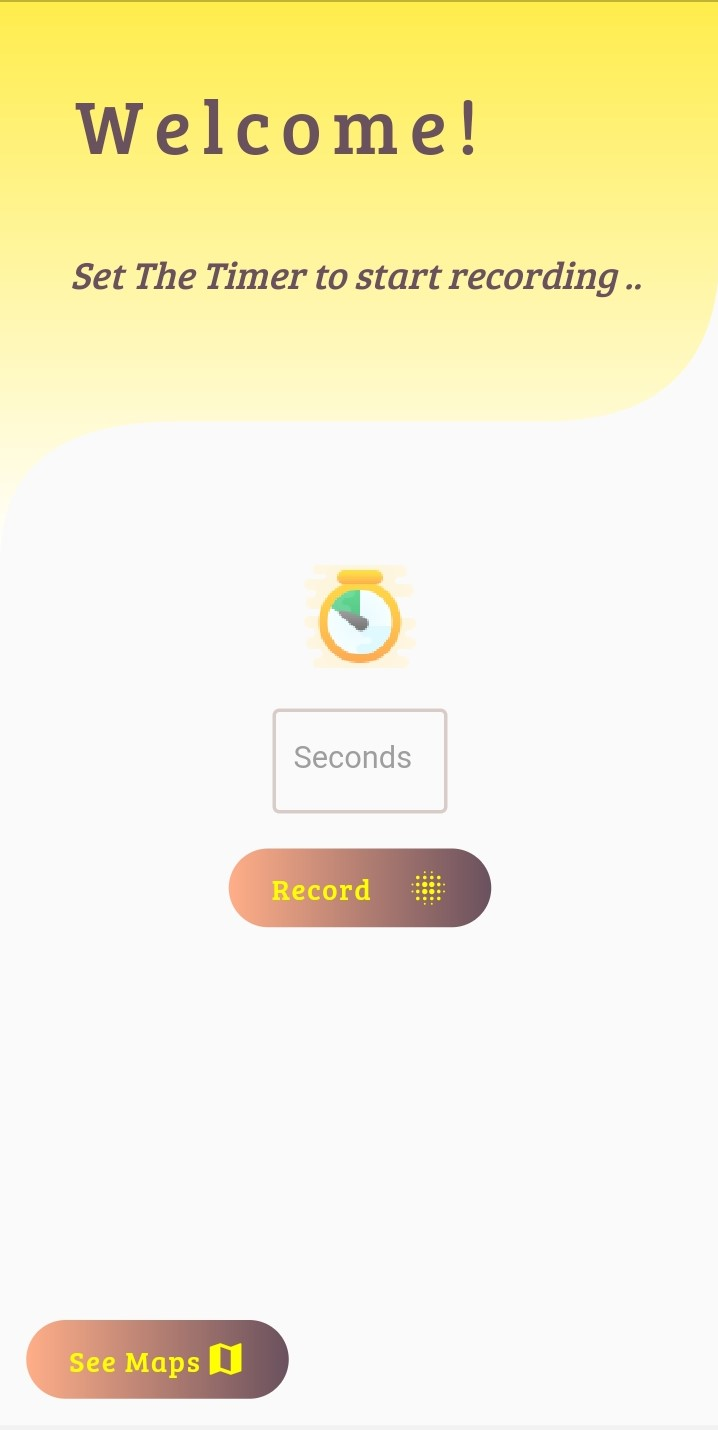
\includegraphics[width=0.8\textwidth]{Images/recordingApp/firstScreen.jpg}
            \caption{Welcome Screen.}
            \label{fig:Welcome Screen}
        \end{subfigure}
        \begin{subfigure}{.49\textwidth}
            \center
            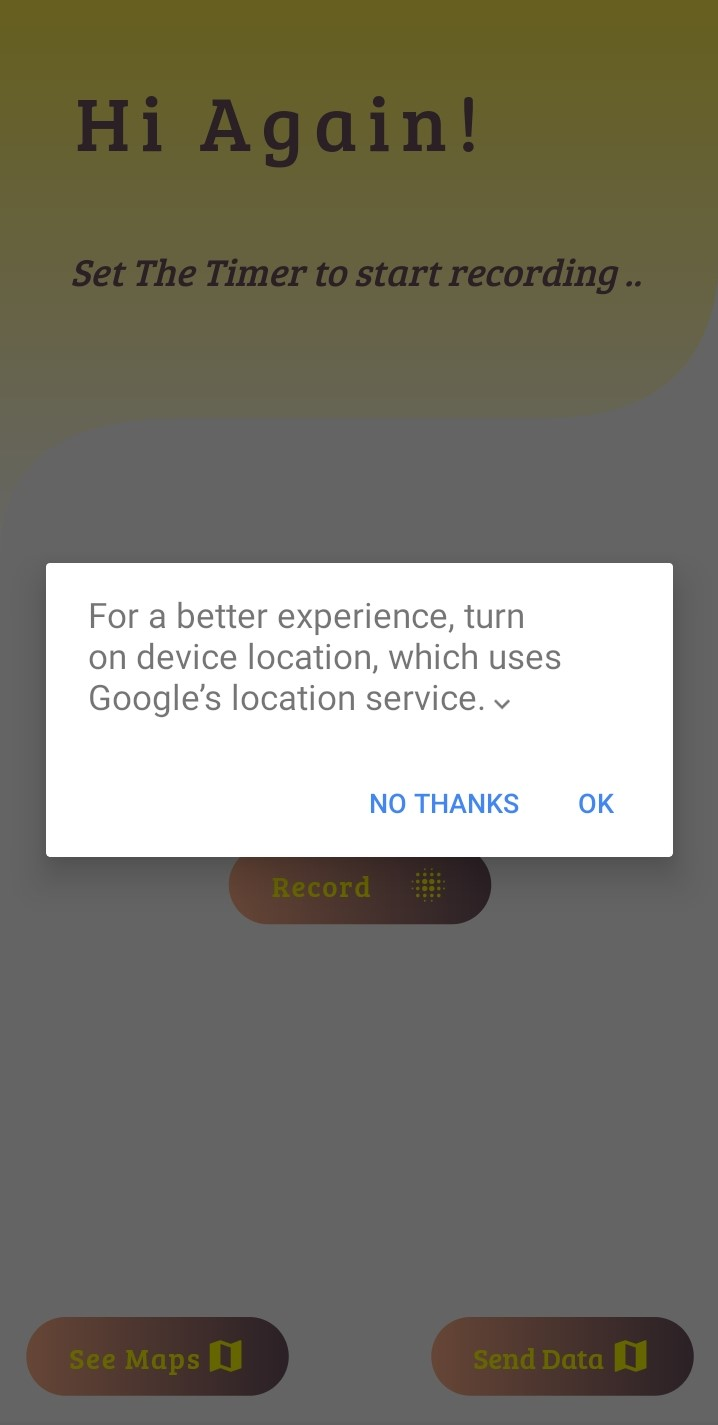
\includegraphics[width=0.8\textwidth]{Images/recordingApp/askingGps.jpg}
            \caption{Gps activating alert.}
            \label{fig:GpsAcivate}
        \end{subfigure}
        \begin{subfigure}{.49\textwidth}
            \center
            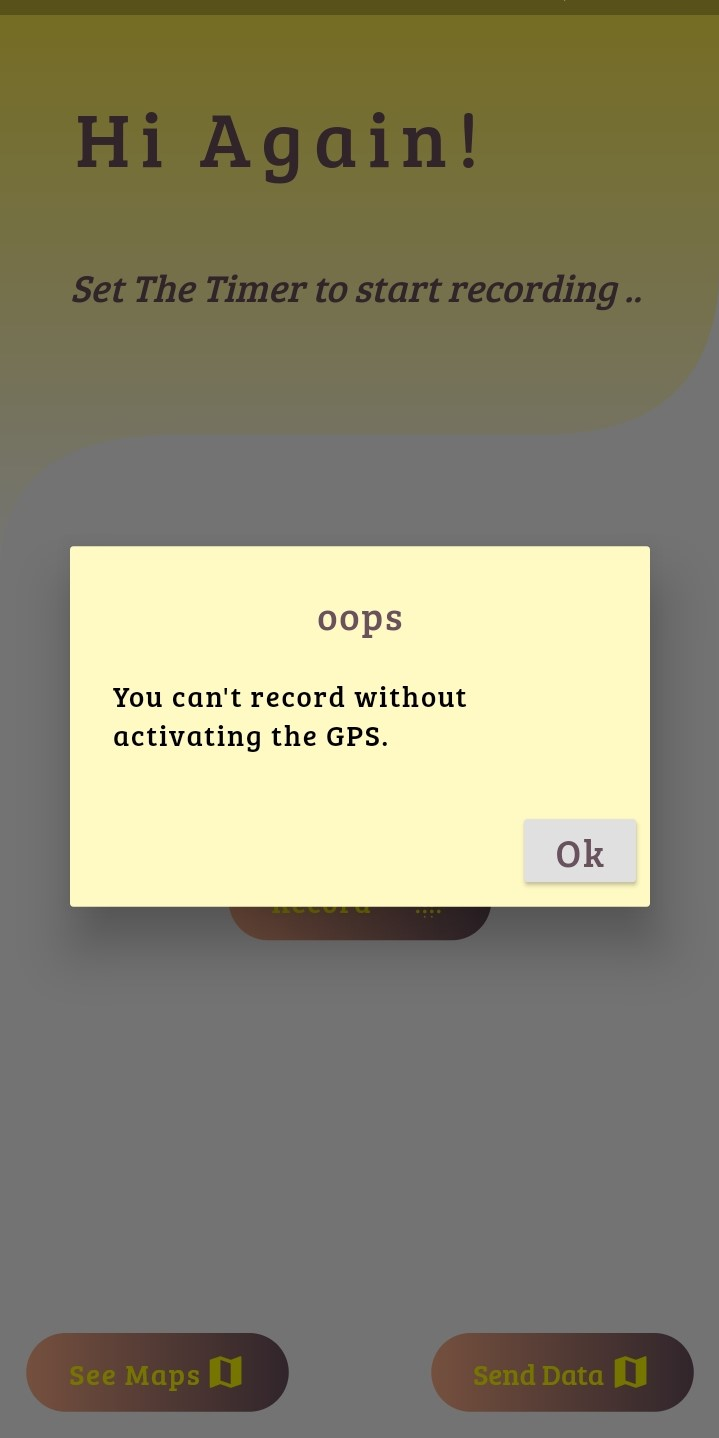
\includegraphics[width=0.8\textwidth]{Images/recordingApp/noGpsAlert.jpg}
            \caption{Notification to ativate GPS.}
            \label{fig:gpsNotif}
        \end{subfigure}
        \begin{subfigure}{.49\textwidth}
            \center
            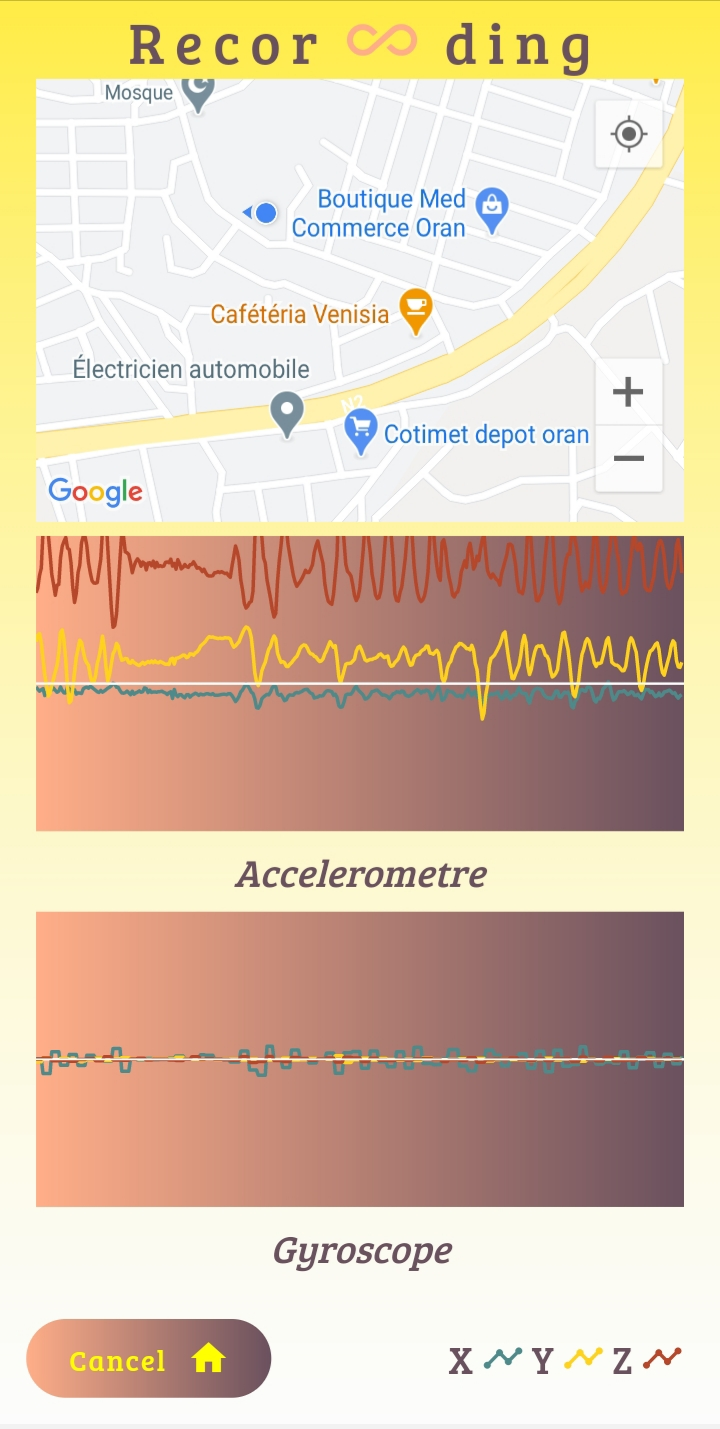
\includegraphics[width=0.8\textwidth]{Images/recordingApp/recordingScreen.jpg}
            \caption{Recording Screen.}
            \label{fig:Recording}
        \end{subfigure}
        \caption{Application de récolte}
        \label{fig:app_recolte}
    \end{figure}

    \item Lorsque le temps est écoulé, l'application envoie des données au serveur une fois que l'utilisateur clique sur «Envoyer les données» - elles seront envoyées automatiquement dans les travaux futurs - (Figure \ref{fig:Done}).
          \begin{figure}[h!]
              \center
              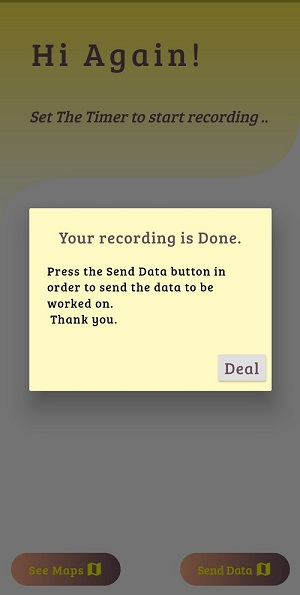
\includegraphics[width=0.50\textwidth]{Images/recordingApp/doneRecording.jpg}
              \caption{Done Recording.}
              \label{fig:Done}
          \end{figure}

          L'application les enregistre également sous forme de fichier CSV contenant  (Figure \ref{fig:csv}).:
          \begin{itemize}
              \item La durée d'enregistrement (Time).
              \item Données de l'accéléromètre (Accel X, Accel Y, Accel Z).
              \item Données du gyroscope (Gyro X, Gyro Y, Gyro Z).
              \item Données GPS (Lat, Long).
              \item Données de la vitesse du véhicule (Speed).
          \end{itemize}
          \begin{figure}[h!]
              \center
              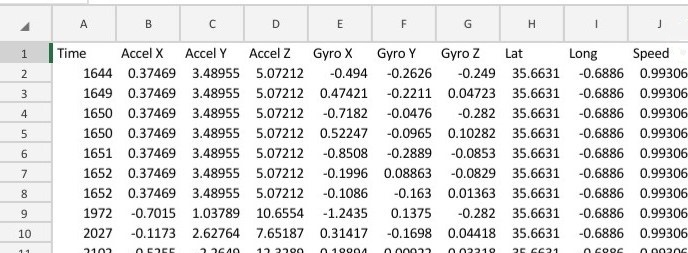
\includegraphics[width=0.75\textwidth]{Images/recordingApp/csv.jpg}
              \caption{CSV File.}
              \label{fig:csv}
          \end{figure}



\end{itemize}

\newpage

\section{Serveur de traitement}
Un serveur informatique est un dispositif informatique (matériel et logiciel) qui offre des services à un ou plusieurs clients (parfois des milliers).


En fonctionnement, un serveur répond automatiquement à des requêtes provenant d'autres dispositifs informatiques (les clients), selon le principe dit client-serveur. Le format des requêtes et des résultats est normalisé, se conforme à des protocoles réseaux et chaque service peut être exploité par tout client qui met en œuvre le protocole propre à ce service.

Dans notre implémentation, le serveur de traitement prend en charge:
\renewcommand{\labelitemi}{$\bullet$}
\begin{itemize}
    \item Traitez les données avec l'algo comme indiqué au chapitre 3, qui renvoie deux résultats; score et nombre d'anomalies. \textcircled{screenshot of the python code}
    \item Utilise flask pour faire partie de l'API, afin que toutes les autres applications concernées puissent communiquer avec le serveur, notre application principale ici est l'application Flutter (chapitre 4 section kda).
\end{itemize}
\subsection{Avantages de l'API (Application Programming Interface)}
Les API sont conçues pour tirer parti de la puissance de la connectivité. L'utilisation des API a entraîné une croissance considérable pour les entreprises en permettant aux développeurs de gérer les relations de l'entreprise avec les parties prenantes de manière à ce que ces dernières restent informées de tout changement éventuel dans l'ensemble du système. voici quelques avantages non négligeables des intégrations d'API:

\begin{figure}[h!]
    \center
    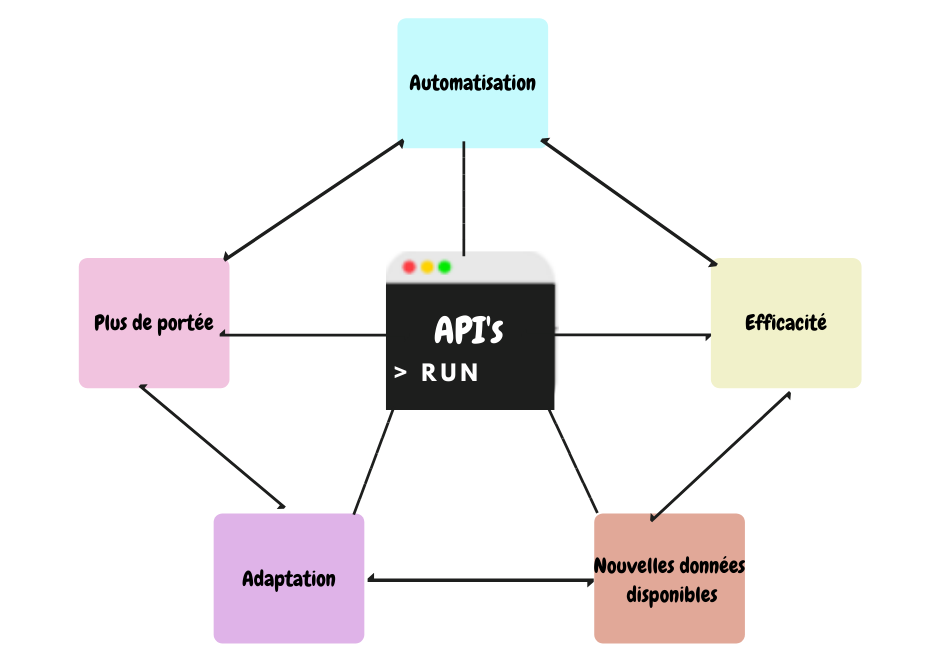
\includegraphics[width=0.75\textwidth]{Images/chapter3/apiAvantages.png}
    \caption{Avantages de l'API}
  \end{figure}


\begin{description}
    \item [Automatisation]: C'est le premier avantage le plus concret de l'utilisation de l'API. Au lieu de personnes, les ordinateurs feront le travail, réduisant ainsi le temps total. Avec l'aide des API, les développeurs peuvent gérer le travail plus rapidement et mettre à jour les flux de travail de manière à devenir plus productifs en peu de temps.
    \item [Plus de portée]: L'ironie derrière l'utilisation de toute interface moderne est de pagayer les informations en peu de temps de la manière la plus sûre possible. En incorporant l'API dans le système, une couche d'application peut aider à distribuer des informations en douceur à d'autres systèmes et à offrir des services à de nouveaux clients. La partie intrigante de cette interface est qu'elle permet aux développeurs de créer un service personnalisé pour de nouveaux publics
     \item[Efficacité] : Une fois que vous avez accès à l'API, il est facile pour le nouveau contenu d'être publié rapidement. Le système publie le contenu automatiquement et le rend disponible pour chaque chaîne. Par conséquent, le contenu est facilement partagé avec un public massif. 
     \item[Adaptation] : Chaque système doit être modifié au fil du temps, et l'API personnalisée aide à changer le système rapidement.
     \item[Nouvelles données disponibles] : La meilleure chose à propos de l'API est sa caractéristique étonnante d'égalité sociale. Chaque fois qu'il y a des informations à partager, l'API les partage avec toutes les parties de la communication.
\end{description} 



  \subsection{Implémentation de l’API}
  Notre API définit principalement 1 ressource : 
 IDUUUNNNNOOO
